% Provenance (never printed): cycle 3 geography and "La planete Terre"
% (the great physical features of the world: relief, rivers, deserts, ice;
% reading a physical map); see sources/book1/PROVENANCE.md.
% Book 1, grade 4, chapter 3.
\chapter{El mapa físico del mundo}\label{ch:g4:world-physical-map}

Sami y Noor despliegan un gran \omterm{def:g2:drawing-to-map:map}{mapa} del mundo en el suelo del aula y se
arrodillan a su alrededor. No se parece a los \omterm{def:g2:drawing-to-map:map}{mapas} que conocen. No hay
países, ni fronteras, ni ciudades. En cambio, la tierra está pintada de
colores: verde a lo largo de las \omterm{def:g1:landscapes-around-us:water}{costas} y en las grandes tierras llanas,
luego amarillo pálido, luego marrón, y en algunos lugares casi blanco.
También el \omterm{def:g2:water-on-earth:ocean}{mar} tiene varios azules: pálido cerca de las \omterm{def:g1:landscapes-around-us:water}{costas}, cada vez más
oscuro \omterm{def:g2:water-on-earth:ocean}{mar} adentro, en los \omterm{def:g2:water-on-earth:ocean}{océanos}.

---¿Por qué esa parte de Asia es blanca? ---pregunta Noor---. ¿Es \omterm{def:g4:clouds-rain-snow:precipitation}{nieve}?
No exactamente. En este \omterm{def:g2:drawing-to-map:map}{mapa}, cada color dice lo alta que está la tierra, o
lo profundo que es el \omterm{def:g2:water-on-earth:ocean}{mar}.

\begin{recall}
Un \omterm{def:g2:drawing-to-map:map}{mapa} muestra un lugar desde arriba, hecho más pequeño; su \omterm{def:g2:drawing-to-map:legend}{leyenda}
explica sus colores y sus signos (\cref{ch:g2:drawing-to-map}). La tierra
firme está reunida en siete \omterm{def:g3:continents-and-oceans:continent}{continentes}, entre cinco \omterm{def:g2:water-on-earth:ocean}{océanos}, y un \omterm{def:g3:continents-and-oceans:world-map}{mapamundi}
es un \omterm{def:g3:continents-and-oceans:globe}{globo} aplanado (\cref{ch:g3:continents-and-oceans}). Las \omterm{def:g1:landscapes-around-us:landform}{montañas}, las
\omterm{def:g1:landscapes-around-us:landform}{colinas}, los \omterm{def:g1:landscapes-around-us:landform}{valles} y las \omterm{def:g1:landscapes-around-us:landform}{llanuras} son las \omterm{def:g1:landscapes-around-us:landform}{formas del relieve}; los \omterm{def:g1:landscapes-around-us:water}{ríos}
bajan de las tierras altas hasta el \omterm{def:g2:water-on-earth:ocean}{mar} (\cref{ch:g1:landscapes-around-us}).
\end{recall}

\section{Leer un mapa físico}

Para decir a qué altura está un lugar, necesitamos un nivel de partida, el
mismo en toda la Tierra. Tomamos el \omterm{def:g4:world-physical-map:altitude}{nivel del mar}.

\begin{definition}[Altitud y nivel del mar]\label{def:g4:world-physical-map:altitude}
El \emph{nivel del mar}\index{nivel del mar} es el nivel medio de la
superficie del \omterm{def:g2:water-on-earth:ocean}{mar}, entre la marea alta y la marea baja. La
\emph{altitud}\index{altitud} de un lugar es su altura sobre el nivel del
\omterm{def:g2:water-on-earth:ocean}{mar}, en metros. Bajo el \omterm{def:g2:water-on-earth:ocean}{mar} hablamos de \emph{profundidad}: a qué distancia
por debajo del nivel del \omterm{def:g2:water-on-earth:ocean}{mar} está el fondo.
\end{definition}

Un pueblo junto al \omterm{def:g2:water-on-earth:ocean}{mar} tiene una \omterm{def:g4:world-physical-map:altitude}{altitud} de unos pocos metros. Un pueblo de
\omterm{def:g1:landscapes-around-us:landform}{montaña} puede estar a 1\,500 metros: kilómetro y medio por encima del \omterm{def:g4:world-physical-map:altitude}{nivel
del mar}, aunque esté a cientos de kilómetros de cualquier \omterm{def:g1:landscapes-around-us:water}{costa}.

\begin{definition}[Relieve]\label{def:g4:world-physical-map:relief}
El \emph{relieve}\index{relieve} de una región es la forma de su tierra:
dónde es alta y dónde es baja, sus \omterm{def:g1:landscapes-around-us:landform}{montañas}, mesetas, \omterm{def:g1:landscapes-around-us:landform}{valles} y \omterm{def:g1:landscapes-around-us:landform}{llanuras}.
\end{definition}

\begin{definition}[Mapa físico]\label{def:g4:world-physical-map:physical-map}
Un \emph{mapa físico}\index{mapa fisico@mapa físico} muestra el \omterm{def:g4:world-physical-map:relief}{relieve} de
la tierra y la profundidad del \omterm{def:g2:water-on-earth:ocean}{mar} con colores, un color para cada escalón
de \omterm{def:g4:world-physical-map:altitude}{altitud} o de profundidad, y también los grandes \omterm{def:g1:landscapes-around-us:water}{ríos}, \omterm{def:g1:landscapes-around-us:water}{lagos}, desiertos y
hielos.
\end{definition}

\begin{omfigure}
\begin{tikzpicture}
\begin{axis}[ommap, width=\linewidth, xtick=\empty, ytick=\empty, grid=none,
    axis background/.style={}, clip=true]
  \addplot graphics[xmin=-180, xmax=180, ymin=-90, ymax=90]
    {figdata/out/grade-4-physical_map.png};
  \addplot[black!45, line width=0.15pt] table {figdata/out/shared-geo-land.dat};
  \addplot[fill=omHypsSeaB, draw=blue!60!black, line width=0.2pt]
    table {figdata/out/grade-4-physical_map-lakes.dat};
  \addplot[blue!70!black, line width=0.5pt] table {figdata/out/grade-4-physical_map-rivers.dat};
  \begin{scope}[every node/.style={font=\scriptsize\bfseries, align=center,
      fill=white, fill opacity=0.7, text opacity=1, inner sep=1pt, rounded corners=1pt}]
    \node at (axis cs:-112,47) {Montañas\\Rocosas};
    \node at (axis cs:-62,-22) {Andes};
    \node at (axis cs:10,49) {Alpes};
    \node at (axis cs:84,24) {Himalaya};
    \node at (axis cs:4,23) {Sáhara};
    \node at (axis cs:-40,74) {Groenlandia\\(hielo)};
    \node at (axis cs:60,-80) {Antártida (hielo)};
  \end{scope}
  \begin{scope}[every node/.style={font=\scriptsize\itshape, text=blue!50!black,
      fill=white, fill opacity=0.6, text opacity=1, inner sep=1pt}]
    \node at (axis cs:38,17) {Nilo};
    \node at (axis cs:-56,-7) {Amazonas};
    \node at (axis cs:-80,33) {Misisipi};
    \node at (axis cs:118,26) {Yangtsé};
  \end{scope}
\end{axis}
\end{tikzpicture}

\smallskip
\begin{tikzpicture}[font=\scriptsize, x=1.18cm]
  \foreach \i/\c/\t in {0/5A9CCF/{más de\\4000}, 1/84BCE0/{2000 a\\4000},
      2/B3D8EE/{200 a\\2000}, 3/DCEEF8/{0 a\\200}} {
    \definecolor{tmp}{HTML}{\c}
    \fill[tmp, draw=black!40] (\i,0) rectangle (\i+0.92,0.35);
    \node[align=center, anchor=north] at (\i+0.45,-0.05) {\t};
  }
  \foreach \i/\c/\t in {5/9CC98A/{0 a\\200}, 6/C9DE99/{200 a\\500},
      7/F1E7A8/{500 a\\1000}, 8/E5C58A/{1000 a\\2000}, 9/C79E76/{2000 a\\4000},
      10/ECE8E3/{más de\\4000}} {
    \definecolor{tmp}{HTML}{\c}
    \fill[tmp, draw=black!40] (\i,0) rectangle (\i+0.92,0.35);
    \node[align=center, anchor=north] at (\i+0.45,-0.05) {\t};
  }
  \node[anchor=south] at (2,0.4) {profundidad del mar (m)};
  \node[anchor=south] at (8,0.4) {altitud de la tierra (m)};
\end{tikzpicture}

{\small El \omterm{def:g4:world-physical-map:physical-map}{mapa físico} del mundo, con su \omterm{def:g2:drawing-to-map:legend}{leyenda}. Cada color es un escalón
de \omterm{def:g4:world-physical-map:altitude}{altitud} (en tierra) o de profundidad (bajo el \omterm{def:g2:water-on-earth:ocean}{mar}). Los \omterm{def:g1:landscapes-around-us:water}{ríos}, en azul
oscuro. El \omterm{def:g4:world-physical-map:relief}{relieve} está dibujado a partir de un valor por cada grado de
latitud y de longitud (más o menos cada 100 kilómetros), así que está
suavizado: no se ven las cumbres aisladas ni las fosas estrechas. Datos:
\omterm{def:g4:world-physical-map:relief}{relieve} NOAA ETOPO1; \omterm{def:g1:landscapes-around-us:water}{ríos}, \omterm{def:g1:landscapes-around-us:water}{lagos} y \omterm{def:g1:landscapes-around-us:water}{costas} de Natural Earth.}
\label{fig:g4:world-physical-map:map}
% ledger: data:etopo1, data:b1-ne-rivers, data:ne-land
\end{omfigure}

\begin{method}[Leer un color en un mapa físico]\label{met:g4:world-physical-map:reading}
Para hallar la \omterm{def:g4:world-physical-map:altitude}{altitud} de un lugar en un \omterm{def:g4:world-physical-map:physical-map}{mapa físico}:
\begin{enumerate}
  \item busca el lugar y fíjate en su color;
  \item busca el mismo color en la \omterm{def:g2:drawing-to-map:legend}{leyenda};
  \item lee el escalón que hay debajo: la \omterm{def:g4:world-physical-map:altitude}{altitud} del lugar está entre los
        dos números.
\end{enumerate}
En el \omterm{def:g2:water-on-earth:ocean}{mar} se hace igual, para la profundidad.
\end{method}

\begin{example}[Tres lugares]\label{ex:g4:world-physical-map:three}
La desembocadura del Amazonas, en la \omterm{def:g1:landscapes-around-us:water}{costa} de América del Sur, es verde
oscuro: su \omterm{def:g4:world-physical-map:altitude}{altitud} está entre 0 y 200 metros. El centro del Sáhara es verde
pálido o amarillo pálido: entre 200 y 1\,000 metros. La meseta que hay al
norte del Himalaya, en Asia, es casi blanca: más de 4\,000 metros.
\end{example}

\section{Las grandes cordilleras}

En el \omterm{def:g2:drawing-to-map:map}{mapa}, los colores marrones y blancos no están repartidos por igual.
Forman franjas largas y estrechas.

\begin{definition}[Cordillera]\label{def:g4:world-physical-map:range}
Una \emph{cordillera}\index{cordillera} es una larga hilera de \omterm{def:g1:landscapes-around-us:landform}{montañas},
unidas entre sí, que se extiende a lo largo de cientos o miles de
kilómetros.
\end{definition}

Los Andes recorren todo el lado oeste de América del Sur. América del Norte
tiene las \omterm{def:g1:landscapes-around-us:landform}{Montañas} Rocosas; Europa, los Alpes; y Asia, la más alta de
todas: el Himalaya. Allí se alza la \omterm{def:g1:landscapes-around-us:landform}{montaña} más alta de la Tierra: el
Everest, de 8\,849 metros de altura, medido de nuevo en 2020.
% ledger: tht:everest

\begin{omfigure}
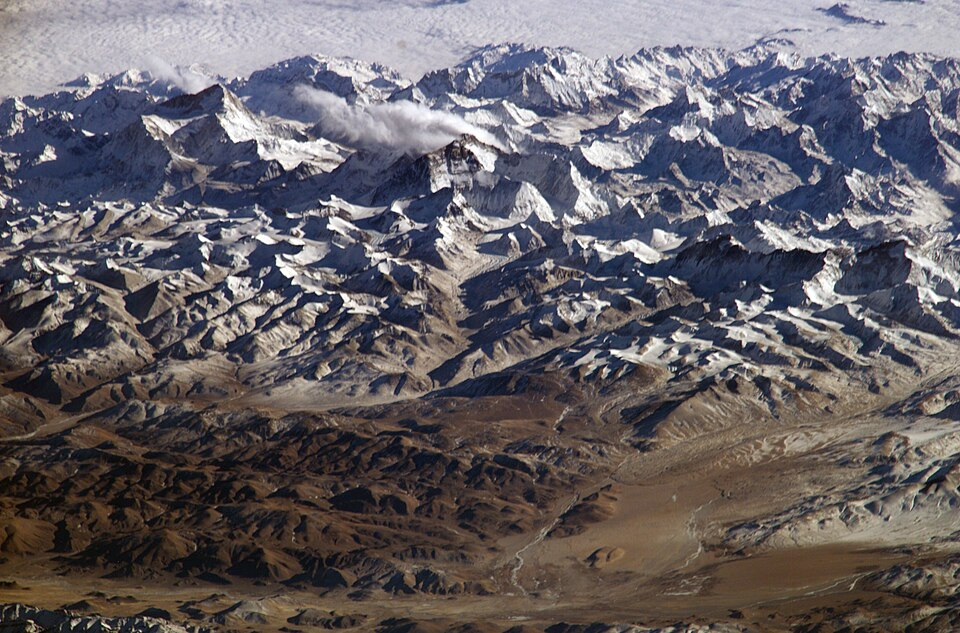
\includegraphics[width=0.75\linewidth]{images/book1/g4-himalaya-iss.jpg}

{\small El Himalaya visto desde la Estación Espacial Internacional,
mirando hacia el sur desde la alta meseta del Tíbet: un \omterm{def:g2:water-on-earth:ocean}{mar} de cumbres
nevadas. Fotografía: NASA (dominio público).}
% ledger: nasa:himalaya-iss
\end{omfigure}

\section{Los grandes ríos y lagos}

La \omterm{def:g4:clouds-rain-snow:precipitation}{lluvia} y la \omterm{def:g4:clouds-rain-snow:precipitation}{nieve} fundida corren por la tierra, se juntan en arroyos y
después en \omterm{def:g1:landscapes-around-us:water}{ríos}, y los \omterm{def:g1:landscapes-around-us:water}{ríos} llevan el agua hasta el \omterm{def:g2:water-on-earth:ocean}{mar}. Los \omterm{def:g1:landscapes-around-us:water}{ríos} más
grandes recogen el agua de regiones enteras de un \omterm{def:g3:continents-and-oceans:continent}{continente}.

Los dos \omterm{def:g1:landscapes-around-us:water}{ríos} más largos de la Tierra son el Nilo, en África, y el Amazonas,
en América del Sur. Cada uno mide cerca de 7\,000 kilómetros. ¿Cuál es el
más largo? Nadie lo sabe con seguridad, porque depende de dónde se decida
que empieza un \omterm{def:g1:landscapes-around-us:water}{río}: entre todos los arroyos que se juntan para formarlo,
¿cuál cuenta como su verdadero comienzo? En 2007, un equipo que siguió el
Amazonas hasta una fuente más lejana dijo que medía unos 6\,800 kilómetros,
un poco más que el Nilo; muchas obras de consulta siguen diciendo que el
Nilo es el más largo.
% ledger: natgeo:nile, natgeo:amazon-nile-2007

El Amazonas es, sin ninguna duda, el \omterm{def:g1:landscapes-around-us:water}{río} más caudaloso: lleva más agua que
ningún otro.
% ledger: natgeo:amazon-nile-2007

\begin{omfigure}
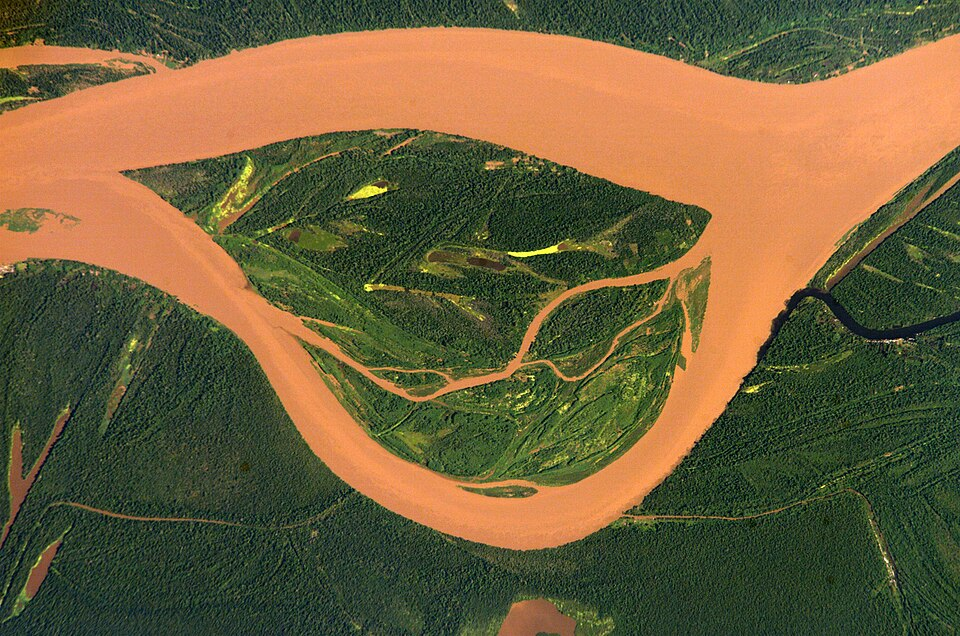
\includegraphics[width=0.6\linewidth]{images/book1/g4-amazon-iss.jpg}

{\small El Amazonas, marrón por el \omterm{def:g3:stones-pebbles-sand:sand}{barro}, serpenteando por la selva, visto
desde la Estación Espacial Internacional. Fotografía: NASA (dominio
público).}
% ledger: nasa:amazon-iss
\end{omfigure}

También los \omterm{def:g1:landscapes-around-us:water}{lagos} baten récords. El \omterm{def:g1:landscapes-around-us:water}{lago} más grande de la Tierra es el mar
Caspio, entre Europa y Asia: es tan grande que se le llama \omterm{def:g2:water-on-earth:ocean}{mar}, pero está
rodeado de tierra por todos los lados. Ocupa más de
370\,000 kilómetros cuadrados. El \omterm{def:g1:landscapes-around-us:water}{lago} más profundo es el \omterm{def:g1:landscapes-around-us:water}{lago} Baikal, en
Rusia: en algunos puntos su fondo está a casi 2 kilómetros por debajo de su
superficie.
% ledger: natgeo:caspian-baikal

\section{Los desiertos y los grandes hielos}

Dos clases de lugares destacan en el \omterm{def:g4:world-physical-map:physical-map}{mapa físico} porque allí no crece casi
nada: los grandes desiertos, donde casi nunca llueve, y los grandes
hielos.

El Sáhara, en el norte de África, es el desierto cálido más grande de la
Tierra. Ocupa unos ocho millones y medio de kilómetros cuadrados. África
entera ocupa unos 30 millones de kilómetros cuadrados, así que el Sáhara es
un poco más de la cuarta parte del \omterm{def:g3:continents-and-oceans:continent}{continente}: más de $\frac{1}{4}$, pero
menos de $\frac{1}{3}$.
% ledger: natgeo:sahara, data:etopo1

Los grandes hielos cubren la Antártida, alrededor del \omterm{def:g3:continents-and-oceans:poles}{Polo Sur}, y casi toda
Groenlandia, en el extremo norte del Atlántico. Allí, la \omterm{def:g4:clouds-rain-snow:precipitation}{nieve} de miles de
años se ha ido amontonando y se ha convertido en una gruesa capa de hielo.
En el \omterm{def:g4:world-physical-map:physical-map}{mapa físico}, sus colores son los de las tierras altas, porque la
superficie del hielo está muy por encima del \omterm{def:g4:world-physical-map:altitude}{nivel del mar}.

\section{Lo más alto y lo más profundo}

El \omterm{def:g4:world-physical-map:physical-map}{mapa físico} muestra la forma de la superficie de la Tierra, pero es tan
pequeño que esconde los extremos. Pongámoslos uno al lado del otro, a
escala.

\begin{omfigure}
\begin{tikzpicture}[x=1cm, y=0.32cm, font=\small]
  % sea level
  \fill[omHypsSeaA] (0,0) rectangle (9,-11.5);
  \fill[omHypsSeaD!80] (4.6,-11.5) -- (4.6,-11.0) -- (5.0,-10.98) -- (5.4,-11.0) -- (5.4,-11.5) -- cycle;
  \draw[black!60] (-0.2,0) -- (9.2,0);
  \node[anchor=west, font=\scriptsize] at (9.25,0) {nivel del mar, 0\,m};
  % height scale
  \draw[black!60] (0,-11.5) -- (0,10);
  \foreach \h in {-10,-8,...,8} {
    \draw[black!60] (-0.1,\h) -- (0,\h);
    \node[anchor=east, font=\scriptsize] at (-0.12,\h) {\h\,km};
  }
  % ocean floor and trench
  \fill[brown!45] (0.05,-11.5) -- (0.05,-3.7) -- (3.2,-3.7) -- (4.4,-6) -- (4.9,-10.98) -- (5.1,-10.98)
    -- (5.6,-6) -- (6.4,-3.7) -- (9,-3.7) -- (9,-11.5) -- cycle;
  \node[font=\scriptsize, align=center] at (2.0,-5.3) {fondo del océano,\\a unos 3\,700\,m};
  \node[font=\scriptsize, anchor=west, align=left] at (5.6,-9.4) {el punto más hondo:\\abismo Challenger,\\casi 11\,000\,m};
  % Everest
  \fill[black!35] (6.6,0) -- (7.6,8.85) -- (8.6,0) -- cycle;
  \fill[white, draw=black!45, line width=0.3pt] (7.35,6.6) -- (7.6,8.85) -- (7.85,6.6) -- (7.6,7.1) -- cycle;
  \node[font=\scriptsize, align=center, anchor=south] at (7.6,8.95) {Everest, 8\,849\,m};
  % cirrus clouds band
  \draw[black!45, line width=0.6pt] (1.0,9.0) .. controls (1.6,9.5) and (2.2,9.1) .. (2.8,9.6);
  \draw[black!45, line width=0.6pt] (1.2,8.3) .. controls (1.8,8.8) and (2.4,8.4) .. (3.0,8.9);
  \node[font=\scriptsize, align=center] at (2.0,7.2) {nubes altas\\(cirros)};
  % a village
  \fill[black!60] (2.2,1.5) rectangle (2.45,1.75);
  \node[font=\scriptsize, anchor=west] at (2.5,1.6) {un pueblo de montaña, 1\,500\,m};
\end{tikzpicture}

{\small Del punto más profundo del \omterm{def:g2:water-on-earth:ocean}{océano} a la cumbre más alta, a escala.
El abismo Challenger, en el \omterm{def:g2:water-on-earth:ocean}{océano} Pacífico, está más hondo bajo el \omterm{def:g2:water-on-earth:ocean}{mar} de
lo que el Everest se eleva por encima de él. Valores: Everest, 8\,849\,m;
abismo Challenger, casi 11\,000\,m; fondo medio del \omterm{def:g2:water-on-earth:ocean}{océano}, unos
3\,700\,m.}
\label{fig:g4:world-physical-map:extremes}
% ledger: tht:everest, usgs:trench-depth, nos:ocean-depth, wmo:cloud-levels
\end{omfigure}

\begin{example}[El Everest en el abismo]\label{ex:g4:world-physical-map:everest-in-deep}
Si pudiéramos levantar el Everest y dejarlo en el fondo del abismo
Challenger, su cumbre seguiría bajo el agua: unos 11\,000 metros de fosa
frente a 8\,849 metros de \omterm{def:g1:landscapes-around-us:landform}{montaña}. Aún lo cubrirían más de 2 kilómetros de
\omterm{def:g2:water-on-earth:ocean}{mar}.
% ledger: tht:everest, usgs:trench-depth
\end{example}

\section{Ejercicios}

\begin{exercise}[$\star$]\label{exo:g4:world-physical-map:1}
¿Qué es la \omterm{def:g4:world-physical-map:altitude}{altitud} de un lugar? ¿Desde qué nivel se mide?
\end{exercise}

\begin{exercise}[$\star$]\label{exo:g4:world-physical-map:2}
Con la \omterm{def:g2:drawing-to-map:legend}{leyenda} del \omterm{def:g4:world-physical-map:physical-map}{mapa físico}, da la \omterm{def:g4:world-physical-map:altitude}{altitud} de un lugar pintado de:
(a) verde oscuro; (b) amarillo pálido; (c) casi blanco.
\end{exercise}

\begin{exercise}[$\star$]\label{exo:g4:world-physical-map:3}
¿En qué \omterm{def:g3:continents-and-oceans:continent}{continente} están: (a) los Andes; (b) el Himalaya; (c) el Sáhara;
(d) las \omterm{def:g1:landscapes-around-us:landform}{Montañas} Rocosas?
\end{exercise}

\begin{exercise}[$\star$]\label{exo:g4:world-physical-map:4}
Nombra la \omterm{def:g1:landscapes-around-us:landform}{montaña} más alta de la Tierra, el \omterm{def:g1:landscapes-around-us:water}{lago} más grande y el \omterm{def:g1:landscapes-around-us:water}{lago} más
profundo.
\end{exercise}

\begin{exercise}[$\star$]\label{exo:g4:world-physical-map:5}
En el \omterm{def:g4:world-physical-map:physical-map}{mapa físico}, el \omterm{def:g2:water-on-earth:ocean}{mar} cerca de las \omterm{def:g1:landscapes-around-us:water}{costas} es azul pálido y el centro de
los \omterm{def:g2:water-on-earth:ocean}{océanos}, azul oscuro. ¿Qué te dice eso sobre la profundidad del \omterm{def:g2:water-on-earth:ocean}{mar}?
\end{exercise}

\begin{exercise}[$\star$]\label{exo:g4:world-physical-map:6}
¿Por qué la Antártida y Groenlandia tienen en el \omterm{def:g4:world-physical-map:physical-map}{mapa físico} el color de
las tierras altas?
\end{exercise}

\begin{exercise}[$\star\star$]\label{exo:g4:world-physical-map:7}
Ordena, del más bajo al más alto: una playa; un pueblo a 1\,500 metros; la
cima del Everest; el fondo del abismo Challenger; el fondo medio del
\omterm{def:g2:water-on-earth:ocean}{océano}.
\end{exercise}

\begin{exercise}[$\star\star$]\label{exo:g4:world-physical-map:8}
¿Por qué no podemos decir con seguridad si el \omterm{def:g1:landscapes-around-us:water}{río} más largo es el Nilo o el
Amazonas?
\end{exercise}

\begin{exercise}[$\star\star$]\label{exo:g4:world-physical-map:9}
África ocupa unos 30 millones de kilómetros cuadrados. ¿Cuánto es la cuarta
parte? ¿Y la tercera parte? El Sáhara ocupa unos ocho millones y medio de
kilómetros cuadrados: ¿es más o menos que la cuarta parte de África? ¿Más o
menos que la tercera parte?
\end{exercise}

\begin{exercise}[$\star\star$]\label{exo:g4:world-physical-map:10}
Un refugio de \omterm{def:g1:landscapes-around-us:landform}{montaña} está a 2\,500 metros, y un \omterm{def:g1:landscapes-around-us:water}{lago}, más abajo, a
1\,000 metros. ¿Cuántos metros más alto está el refugio? ¿De qué colores
son en el \omterm{def:g4:world-physical-map:physical-map}{mapa físico}?
\end{exercise}

\begin{exercise}[$\star\star\star$]\label{exo:g4:world-physical-map:11}
Un avión vuela a 10 kilómetros por encima del \omterm{def:g4:world-physical-map:altitude}{nivel del mar}. ¿Está más alto
que el Everest? ¿Por cuántos metros? Si volara sobre el abismo Challenger,
¿a qué distancia estaría del fondo de la fosa (toma 11\,000 metros para la
fosa)?
\end{exercise}
